% Options for packages loaded elsewhere
\PassOptionsToPackage{unicode}{hyperref}
\PassOptionsToPackage{hyphens}{url}
%
\documentclass[12pt,a4paper]{article}

\usepackage{lmodern}
\usepackage{amssymb,amsmath}
\usepackage{ifxetex,ifluatex}
\ifnum 0\ifxetex 1\fi\ifluatex 1\fi=0 % if pdftex
\usepackage[T1]{fontenc}
\usepackage[utf8]{inputenc}
\usepackage{textcomp} % provide euro and other symbols
\else % if luatex or xetex
\usepackage{unicode-math}
\defaultfontfeatures{Scale=MatchLowercase}
\defaultfontfeatures[\rmfamily]{Ligatures=TeX,Scale=1}
\fi
% Use upquote if available, for straight quotes in verbatim environments
\IfFileExists{upquote.sty}{\usepackage{upquote}}{}
\IfFileExists{microtype.sty}{% use microtype if available
	\usepackage[]{microtype}
	\UseMicrotypeSet[protrusion]{basicmath} % disable protrusion for tt fonts
}{}
\makeatletter
\@ifundefined{KOMAClassName}{% if non-KOMA class
	\IfFileExists{parskip.sty}{%
		\usepackage{parskip}
	}{% else
		\setlength{\parindent}{0pt}
		\setlength{\parskip}{6pt plus 2pt minus 1pt}}
}{% if KOMA class
	\KOMAoptions{parskip=half}}
\makeatother
\usepackage{xcolor}
\IfFileExists{xurl.sty}{\usepackage{xurl}}{} % add URL line breaks if available
\IfFileExists{bookmark.sty}{\usepackage{bookmark}}{\usepackage{hyperref}}
\hypersetup{
	pdftitle={Ideas for the Linac3 Source ML Analysis},
	pdfauthor={Max Mihailescu},
	hidelinks,
	pdfcreator={LaTeX via pandoc}}
\usepackage{graphicx}
\makeatletter
\def\maxwidth{\ifdim\Gin@nat@width>\linewidth\linewidth\else\Gin@nat@width\fi}
\def\maxheight{\ifdim\Gin@nat@height>\textheight\textheight\else\Gin@nat@height\fi}
\makeatother
% Scale images if necessary, so that they will not overflow the page
% margins by default, and it is still possible to overwrite the defaults
% using explicit options in \includegraphics[width, height, ...]{}
\setkeys{Gin}{width=0.8\maxwidth,height=\maxheight,keepaspectratio}
% Set default figure placement to htbp
\makeatletter
\def\fps@figure{htbp}
\makeatother
\setlength{\emergencystretch}{3em} % prevent overfull lines
\providecommand{\tightlist}{%
	\setlength{\itemsep}{0pt}\setlength{\parskip}{0pt}}
\setcounter{secnumdepth}{-\maxdimen} % remove section numbering
\newlength{\cslhangindent}
\setlength{\cslhangindent}{1.5em}
\newenvironment{cslreferences}%
{\setlength{\parindent}{0pt}%
	\everypar{\setlength{\hangindent}{\cslhangindent}}\ignorespaces}%
{\par}

\usepackage[margin=2.5cm]{geometry}
\usepackage[margin=1cm, font=small]{caption}

\usepackage[backend=biber]{biblatex} 
\bibliography{bibliography.bib}

\title{Ideas for the Linac3 Source ML Analysis}
\author{Max Mihailescu}
\date{}

\begin{document}
\maketitle

This document provides a collection of ideas and topics for the analysis
of the Linac3 Ion Source from a ML viewpoint. I will try to collect
descriptions and links to interesting papers and summarize the results I
had when trying out some of them.

\hypertarget{clustering}{%
\section{Clustering}\label{clustering}}

Given a collection of data points, clustering is to group together
points that are similar under some kind of similarity metric. Usually,
this is an unsupervised technique, meaning that no reference labels are
known. There exist a variety of different algorithms, and each algorithm
can produce very different results on the same set of data. Therefore it
is crucial to somehow evaluate the results.

For Linac3 we performed a Clustering Analysis with the goal, to see, if
certain settings of the source would lead to a stable beam current. For
the resulting report please contact Detlef Küchler (CERN BE-ABP-HSL).

The clustering algorithm we used is called \emph{Optigrid} and is
described in the paper ``Optimal Grid-Clustering: Towards Breaking the
Curse of Dimensionality in High-Dimensional Clustering'' by Alexander
Hinneburg and Daniel A. Keim~\cite{Hinneburg:OptimalGridClustering}.

\hypertarget{matrix-profile}{%
\section{Matrix Profile}\label{matrix-profile}}

The Matrix Profile is a tool for efficient motif discovery in time
series, i.e.~for discovery of repeated or ``conserved'' patterns. It can
also be used to find time series discords, i.e.~anomalies. A large
number of papers was published by the same working group, you can find
the projects website here~\cite{Keogh:UCRMatrixProfile}. For a good introduction with
example applications read the first paper~\cite{Yeh:MatrixProfileI}.

\hypertarget{what-is-the-matrix-profile}{%
\subsection{What is the Matrix Profile?}\label{what-is-the-matrix-profile}}

First, let's understand what a subsequence is. Consider a time series
\(T=T_1 \dots T_n,\quad T_i\in\mathbb{R}\) of length \(n\), and fix a
number \(m < n\) (typically \(m \ll n\)). Now, a subsequence of length
\(m\) starting at \(i\) is the continuous block \(T_i \dots T_{i+m}\).
By sliding a window of size \(m\) over \(T\) we can get all \(n-m+1\)
subsequences of length \(m\).

Now, we can define the distance between two subsequences. The most
obvious choice is the euclidean distance
\(dist(Q, T) = \sqrt{\left(Q_1 - T_1\right)^2+\dots+\left(Q_m-T_m\right)^2}\).
However, for the matrix profile we work with the so called
\emph{z-normalized} euclidean distance. It is the euclidean distance of
the z-normalized subsequences, i.e.~we subtract the mean of the
subsequence and divide the difference by the subsequence' standard
deviation, and only then take the euclidean distance. By this we rescale
all subsequences to make them more compareable. Note that under some
circumstances this might be undesirable, for example when search for
motifs in the call of a bird where the pitch could be relevant, and not
only the shape of a signal.

The Matrix Profile \(P\) is a meta time series, that for every
subsequence stores the smallest distance to some other subsequence.
Furthermore, the Matrix Profile Indices \(I\) is another meta time
series, that for every subsequence stores the starting index of the
subsequence, that has the smallest distance to it (its nearest
neighbor). If you imagine the subsequences being points in a \(m\)
dimensional Space, then the matrix profile index of a subsequence is the
starting index of the closest neighbor and the matrix profile value is
the distance to the closest neighbor.

\begin{figure}
\centering
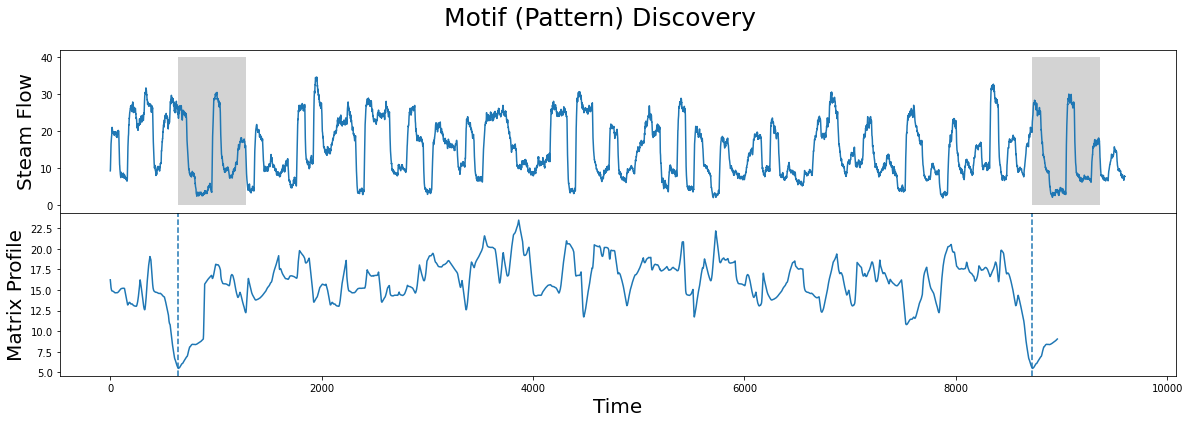
\includegraphics{images/MP_example.png}
\caption{Example of the matrix profile on the steamgen dataset.}
\end{figure}

So, what does this tell us? In the example above you can see a
visualization of the Matrix Profile for the
\href{https://www.cs.ucr.edu/~eamonn/iSAX/steamgen.dat}{Steamgen
Dataset}. In the upper plot you see the data set, and in the lower plot
you see a plot of the Matrix Profile. The two dashed lines represent the
lowest values in the Matrix Profile. This means the two subsequences
that start at each of these lines have a very small (the smallest)
distance from each other, hence they are very similar. This means, that
by visually inspecting the Matrix Profile we can immediately see the
most repeated pattern. There are various other things to discover and
better overview can be found on the UCR page~\cite{Keogh:UCRMatrixProfile}. There exist
also generalizations to more dimensions, see~\cite{Yeh:MatrixProfileVI}.

There exists a very good Python library called \emph{stumpy} for
computing the Matrix Profile that also has very good support by the
author. The Github page can be found here~\cite{Law:stumpy}.

\hypertarget{how-could-the-mp-be-used}{%
\subsection{How could the MP beused?}\label{how-could-the-mp-be-used}}

As described above, the MP profile is a tool that can help to discover
repeating or anomalous patterns in time series data. Hence we can aim to
apply it to any of the many time series produced by the source.

\begin{enumerate}
\def\labelenumi{\arabic{enumi}.}
\tightlist
\item
  Patterns in the BCT currents for prediction: One could try to discover
  repeating patterns in the BCT currents and see if they can be used to
  predict the future development. For example if a pattern indicates a
  degradation of the current in the near future, it could be used to
  alert the operators in time. There exists also a real time version of
  the MP, where it gets updated with every arriving data point. For this
  the SDTS algorithm~\cite{Yeh:MatrixProfileIV} built on top of
  the MP could be interesting.
\item
  Pattern in the BCT current for analysis: Likewise, one could try to
  link patterns in the BCT with patterns/actions of other parameters.
  For example, often times a slow increase of the HT current leads to a
  slow degradation of the BCT current.
\item
  Motifs of different parameter combinations shifted in time: When
  computing the multidimensional matrix profile, to see if there are
  motifs in more than on dimension, one could shift one of the time
  series in time, to see for example how a change of the gas voltage
  affects the current in one hour.
\item
  Meta time series: Instead of looking at the original time series, one
  could try to look for motifs or discords in a rolling window time
  series. For example, one could calculate the standard deviation in one
  hour windows over the BCT25 current and look for repeated patterns
  there, to maybe find motifs that will indicate a future unstable
  period.
\end{enumerate}

\hypertarget{difficulties}{%
\subsection{Difficulties}\label{difficulties}}

The MP is built under the assumption, that repeated patterns or motifs
are an effect of a regular event in the generating process. One example
from the Papers is Seismology. There the time series is the recording of
a Seismograph, which can have very long periods of ``random'' data,
where nothing happens. However, an earthquake would show up with a very
distinctive shape.

\begin{figure}
\centering
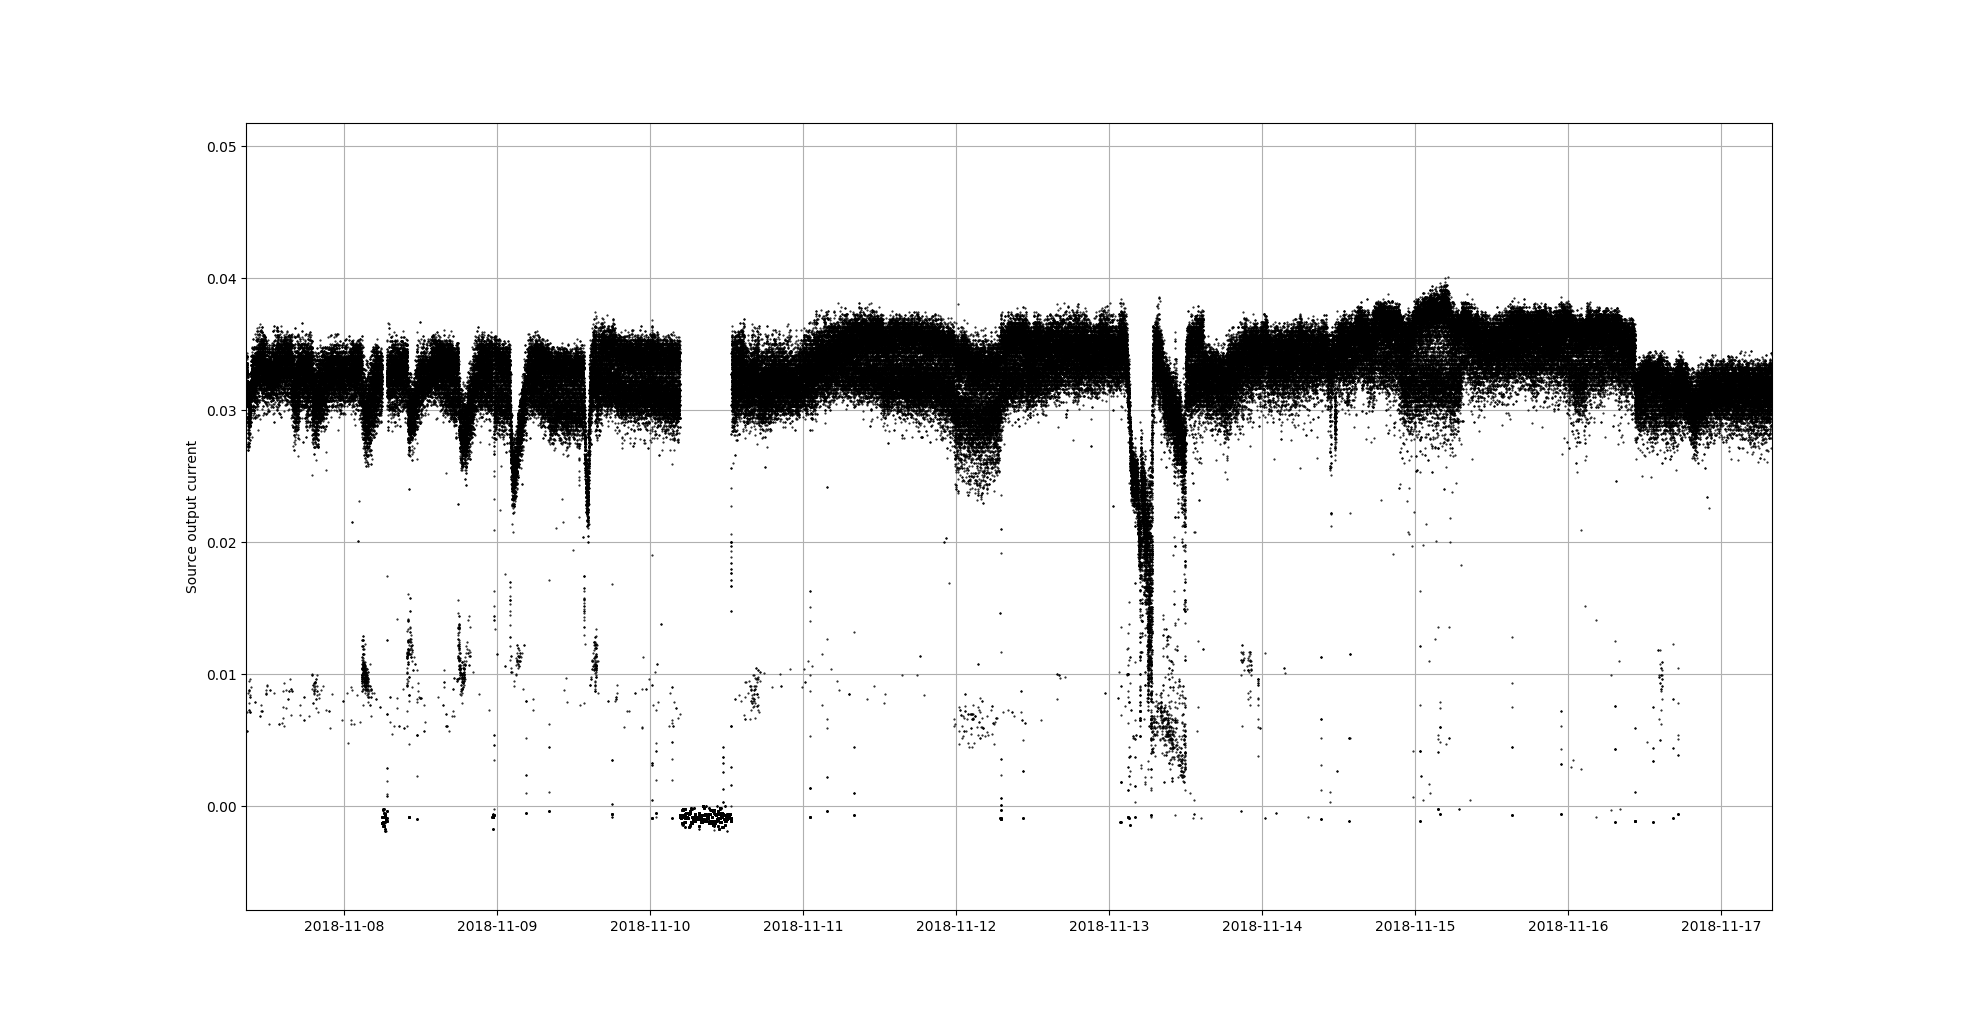
\includegraphics{images/current_demo.png}
\caption{Example of the BCT25 current}
\end{figure}

\begin{figure}
\centering
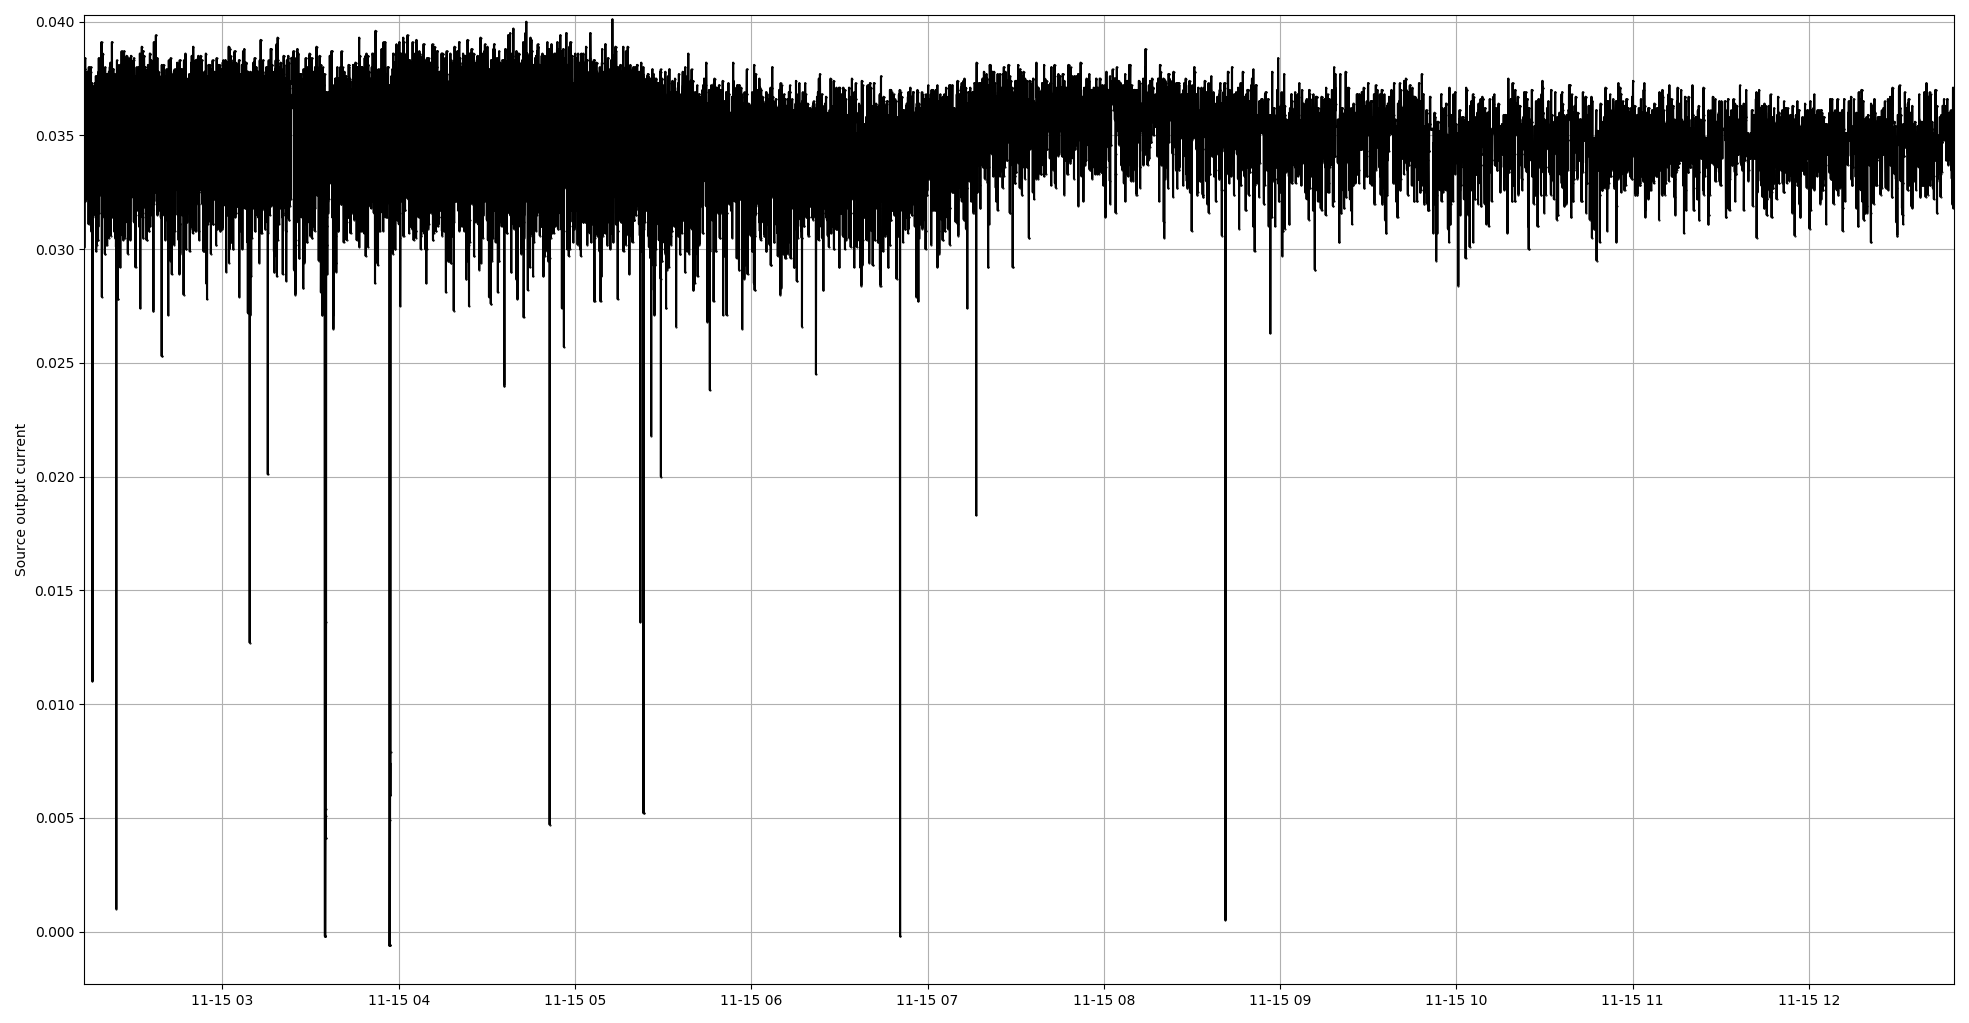
\includegraphics{images/current_demo_2.png}
\caption{Example of the BCT25 current, smaller window}
\end{figure}

In our case however, the BCT signals are mostly flat with oscillations
(see the two images above), hence motif discovery with z-normalized
subsequences is very insufficient. If you have two flat signals with a
lot of added noise, their z-normalized euclidean distance will be very
large, even if one might expect it to be small because visually they are
very similar. There are some ideas to mitigate the problem~\cite{Paepe:EliminatingNoiseMatrix}, 
but I didn't get any satisfying results.

\hypertarget{results}{%
\subsection{Results}\label{results}}

Instead of trying to use a matrix profile with removed noise I flattened
the signal over some minutes and found several links of parameter
changes to BCT current. The results where achieved using the MSTOMP
algorithm~\cite{Yeh:MatrixProfileVI}, a multi dimensional
generalisation of the matrix profile calculation.

\begin{figure}
\centering
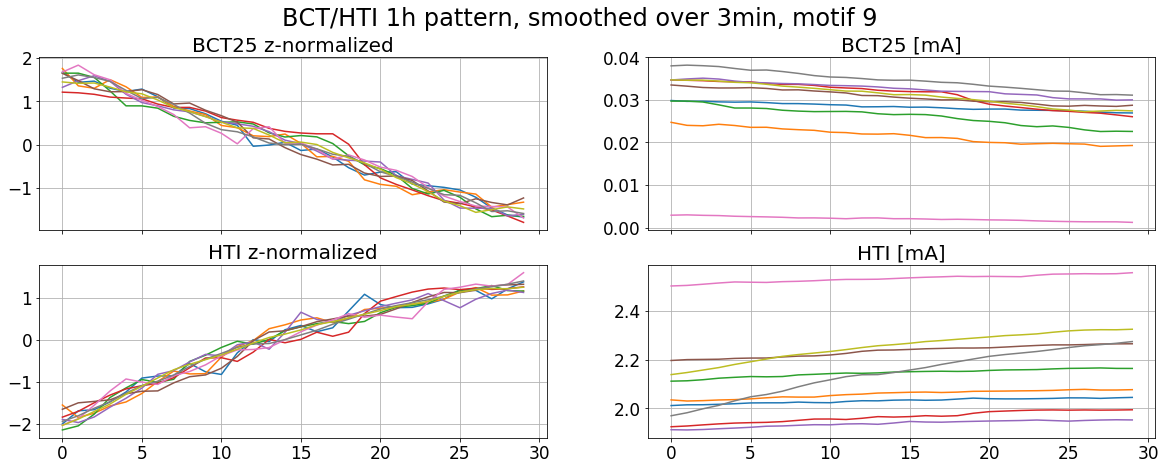
\includegraphics{images/hti_bct_htirise.png}
\caption{Rise of HTI (bottom) and degradation of BCT25 current (top).}
\end{figure}

A rising HTI often coincides with a degrading BCT25 current, so this
seems to confirm this theory. However it is not a proof that an opposite
effect (e.g.~rising HTI and rising BCT current) doesn't also exist. But
we didn't observe it in the time frame we considered (August and
September 2016).

\begin{figure}
\centering
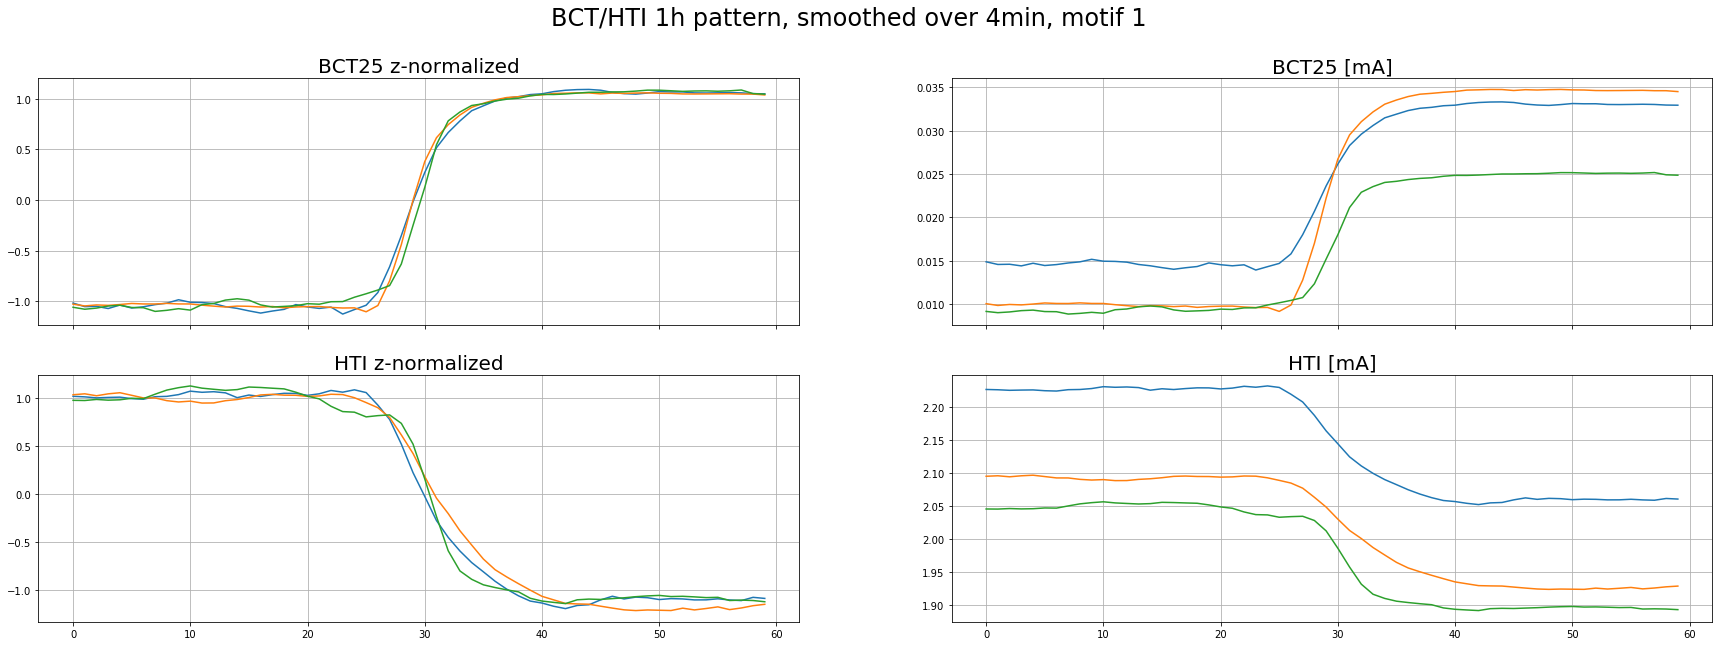
\includegraphics{images/hti_bct_htifall.png}
\caption{Drops of the HTI and jumps in the BCT25 current.}
\end{figure}

The reverse can also be seen. Drops of the HTI correlate with jumps in
the BCT25 current.

\begin{figure}
\centering
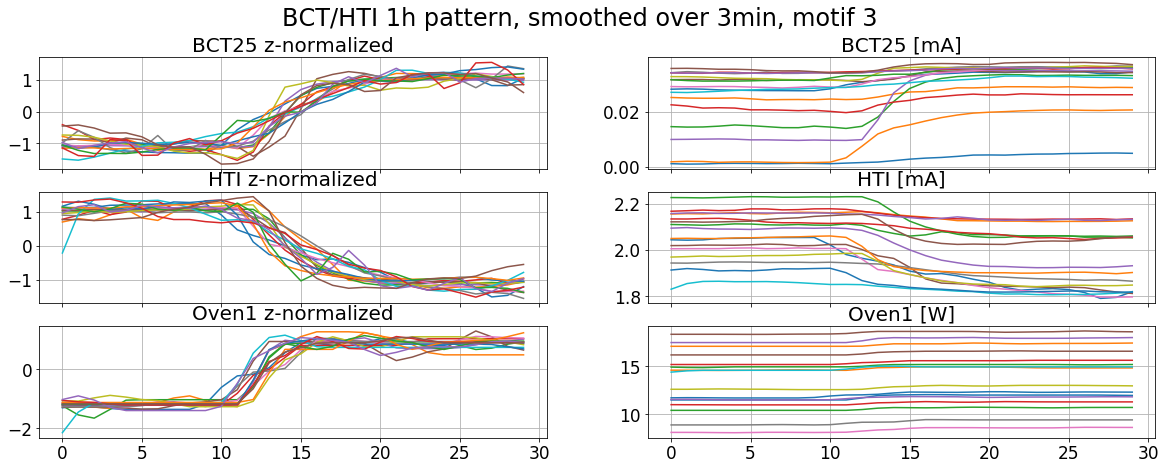
\includegraphics{images/bct_oven_hti.png}
\caption{A common pattern when including BCT25 current, HTI and Oven1
power.}
\end{figure}

One possible explanation we explored is that the behavior in the second
image can often time be achieved by increasing the Oven Power. This can
be seen in this image.

\begin{figure}
\centering
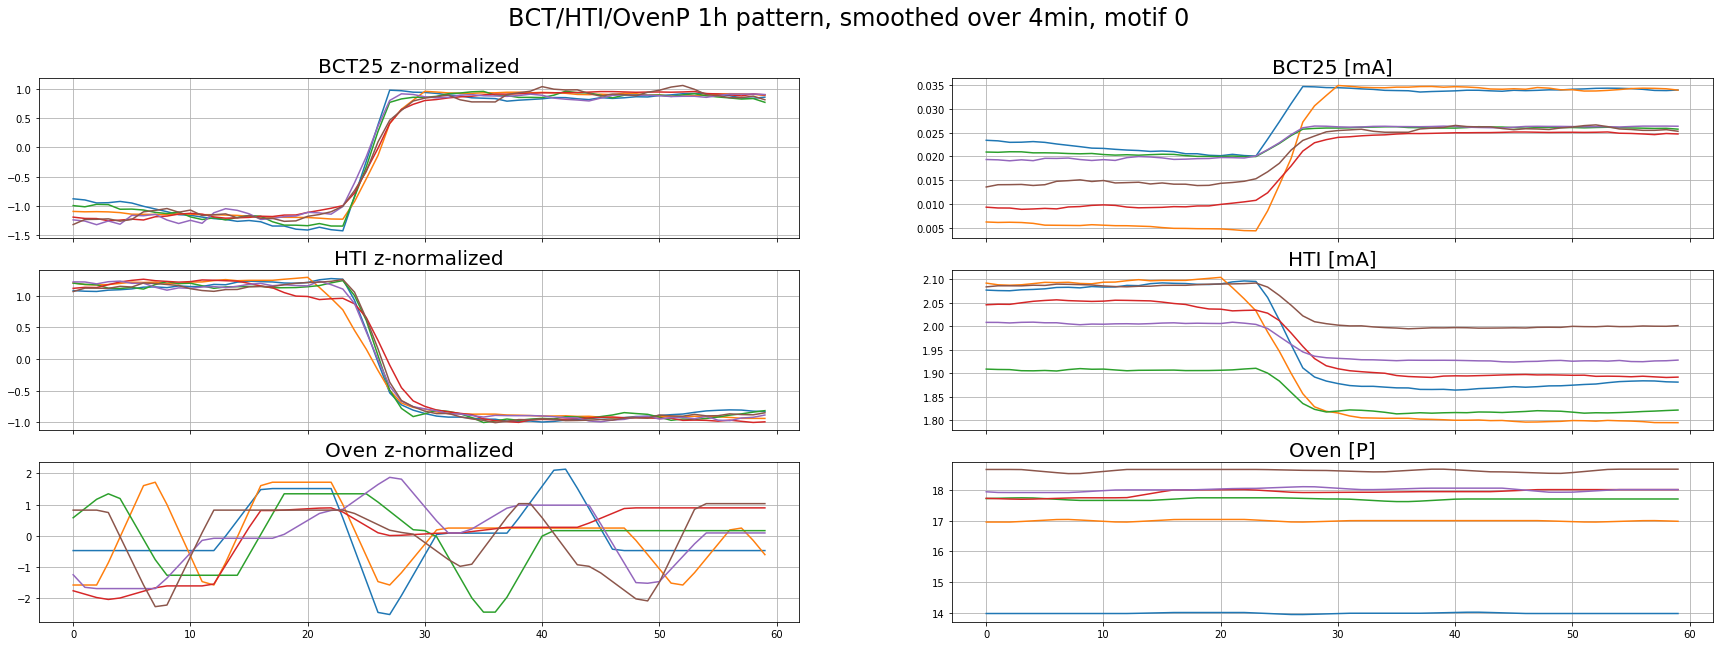
\includegraphics{images/bct_oven_hti_2dim.png}
\caption{Jumps in BCT25 current and HTI without changes of the Oven
power.}
\end{figure}

However, it appears that there are cases where the oven remains
unchanged. Further invastigation is necessary, but it could be that the
power of Oven 2 was increased, as this is only the data for Oven 1.

\begin{figure}
\centering
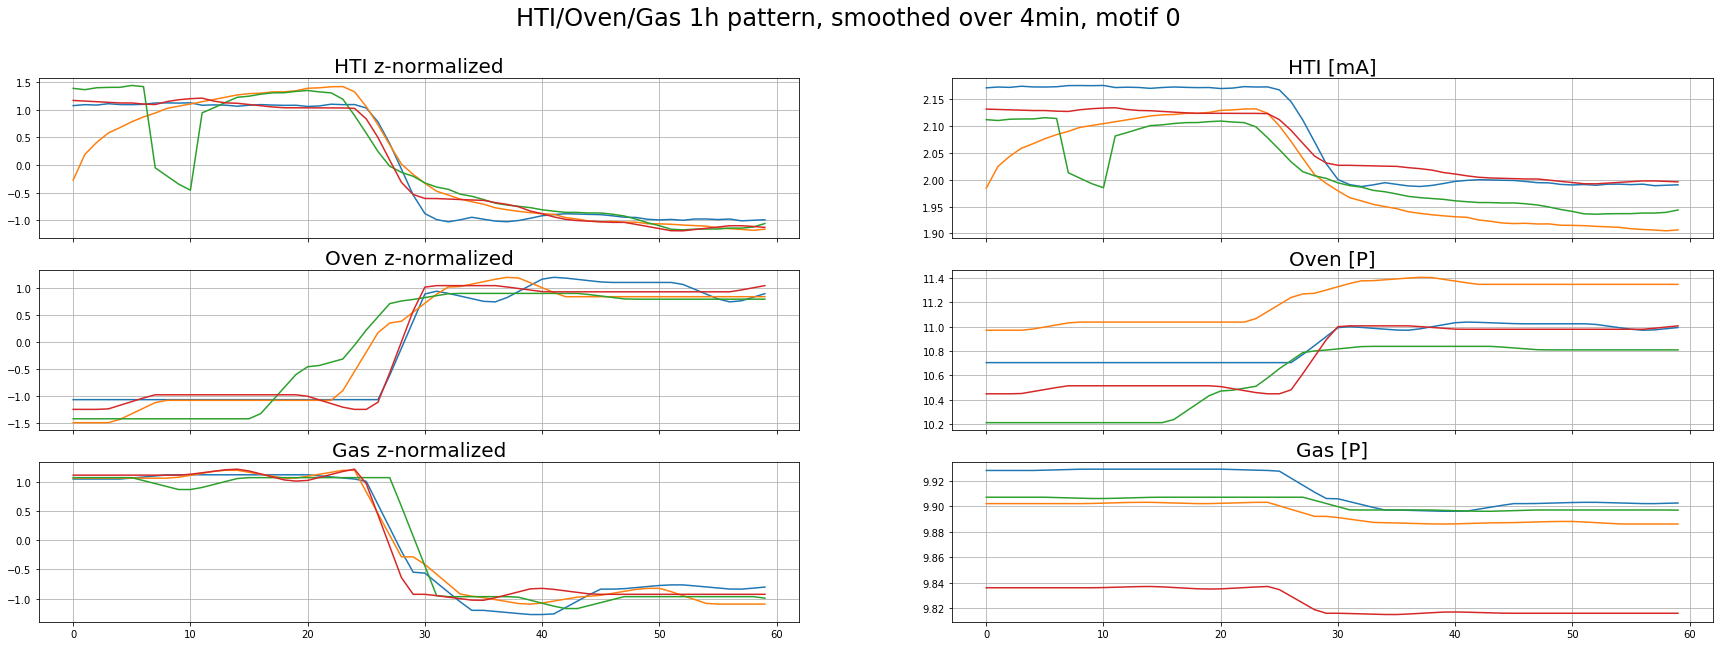
\includegraphics{images/gas_oven_hti.png}
\caption{Correlation of gas voltage decreases with oven power
increases.}
\end{figure}

We could also see that an increase of the oven power is often
accompanied with a decrease of the gas voltage.

We didn't see any meaningful motifs when jointly looking at the Bias
Disc Voltage and the BCT25 current.

\hypertarget{discretization}{%
\section{Discretization}\label{discretization}}

One problem of using the data from CALS/NXCALS is that for all setting
only acquisitions are logged. This means, that we typically don't know
the exact values a setting was changed to, see the figure below for
example. It shows one day (05.11.2018) of Oven1 power acquisition from
NXCALS, where only one data point every five minutes is logged. From the
logbook we can learn that at 14:00 the Oven1 Power was set to 12.0W,
however on the plot we can see some oscillations (The times in the plot
are UTC, so you have to count +2h).

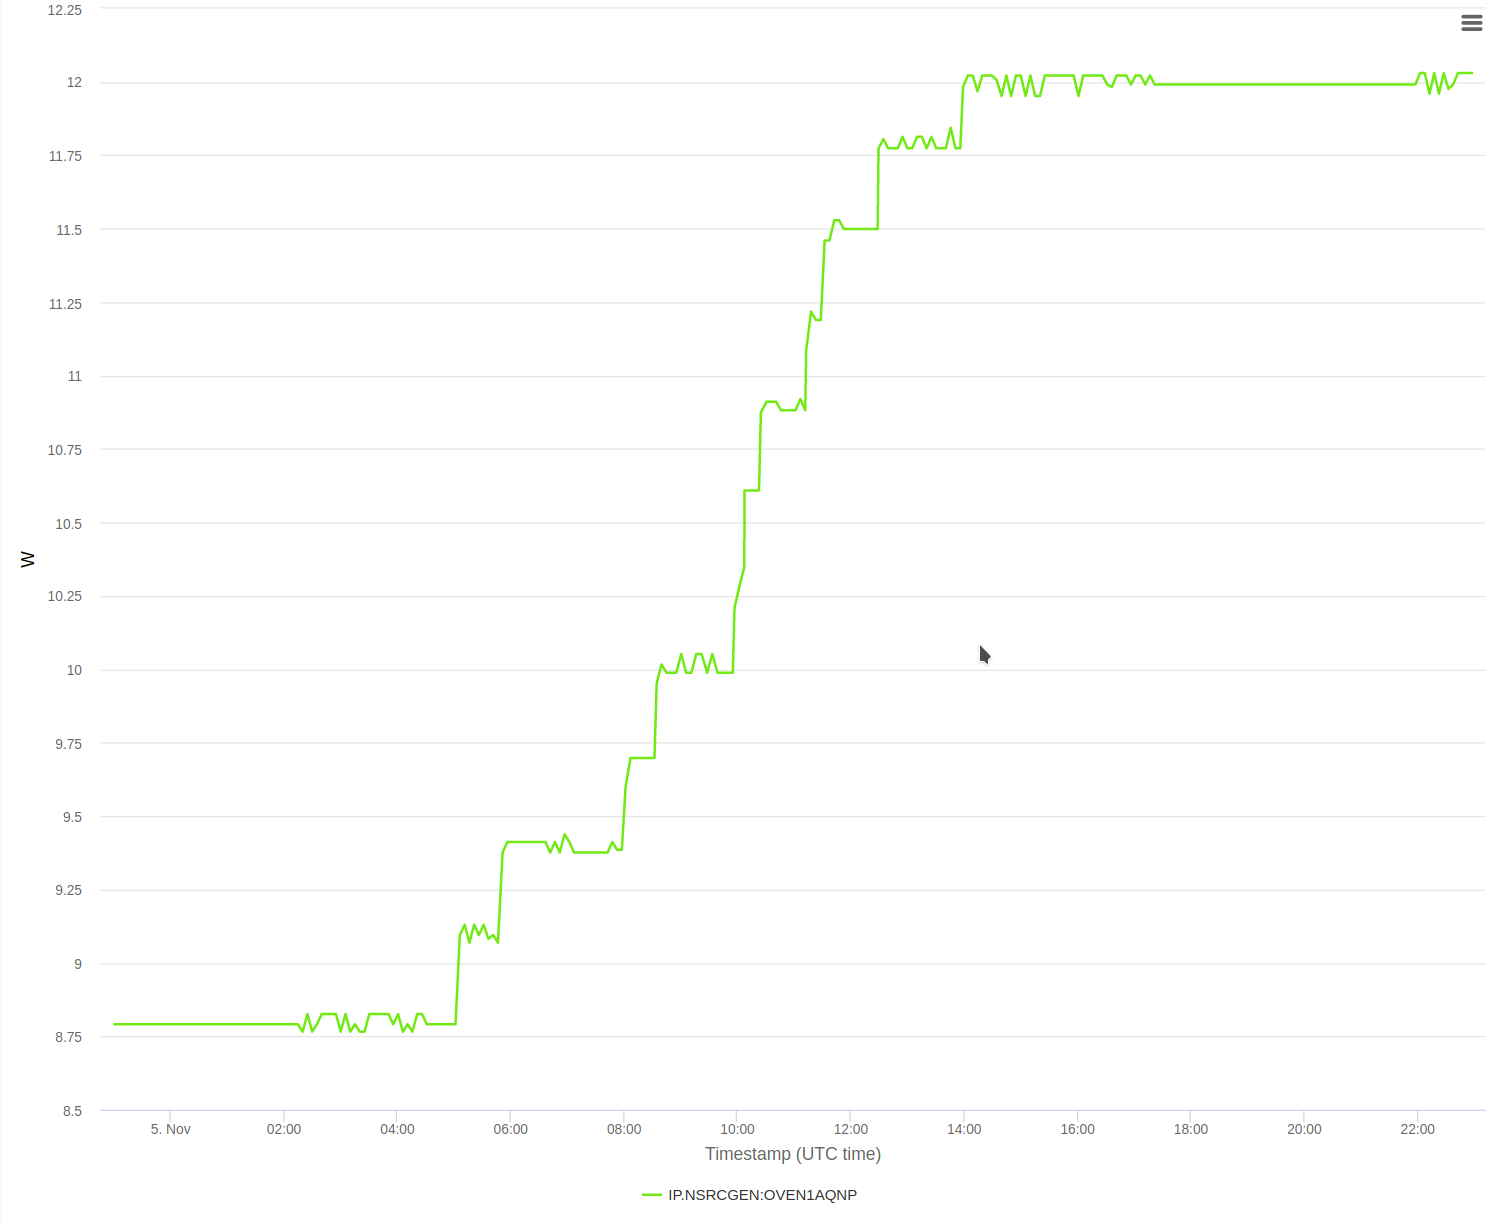
\includegraphics{images/oven1example_05112018.png}

\begin{figure}
\centering
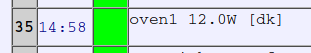
\includegraphics{images/oven1example_logbook_05112018.png}
\caption{Top: Screenshot of Oven1 Acquisition, Bottom: The real value
that was set at 14:00.}
\end{figure}

The same occurs with other settings, and raises the problem that we
cannot directly say when a change of a certain setting happened. So I
tried to discretize the raw acquisition values and get back the true
setting where possible. The main assumption I had to make is that a
setting remained constant over time, unless somebody changes it. This
appears reasonable in most cases, but in some extreme cases some
information might be lost (see below).

\begin{figure}
\centering
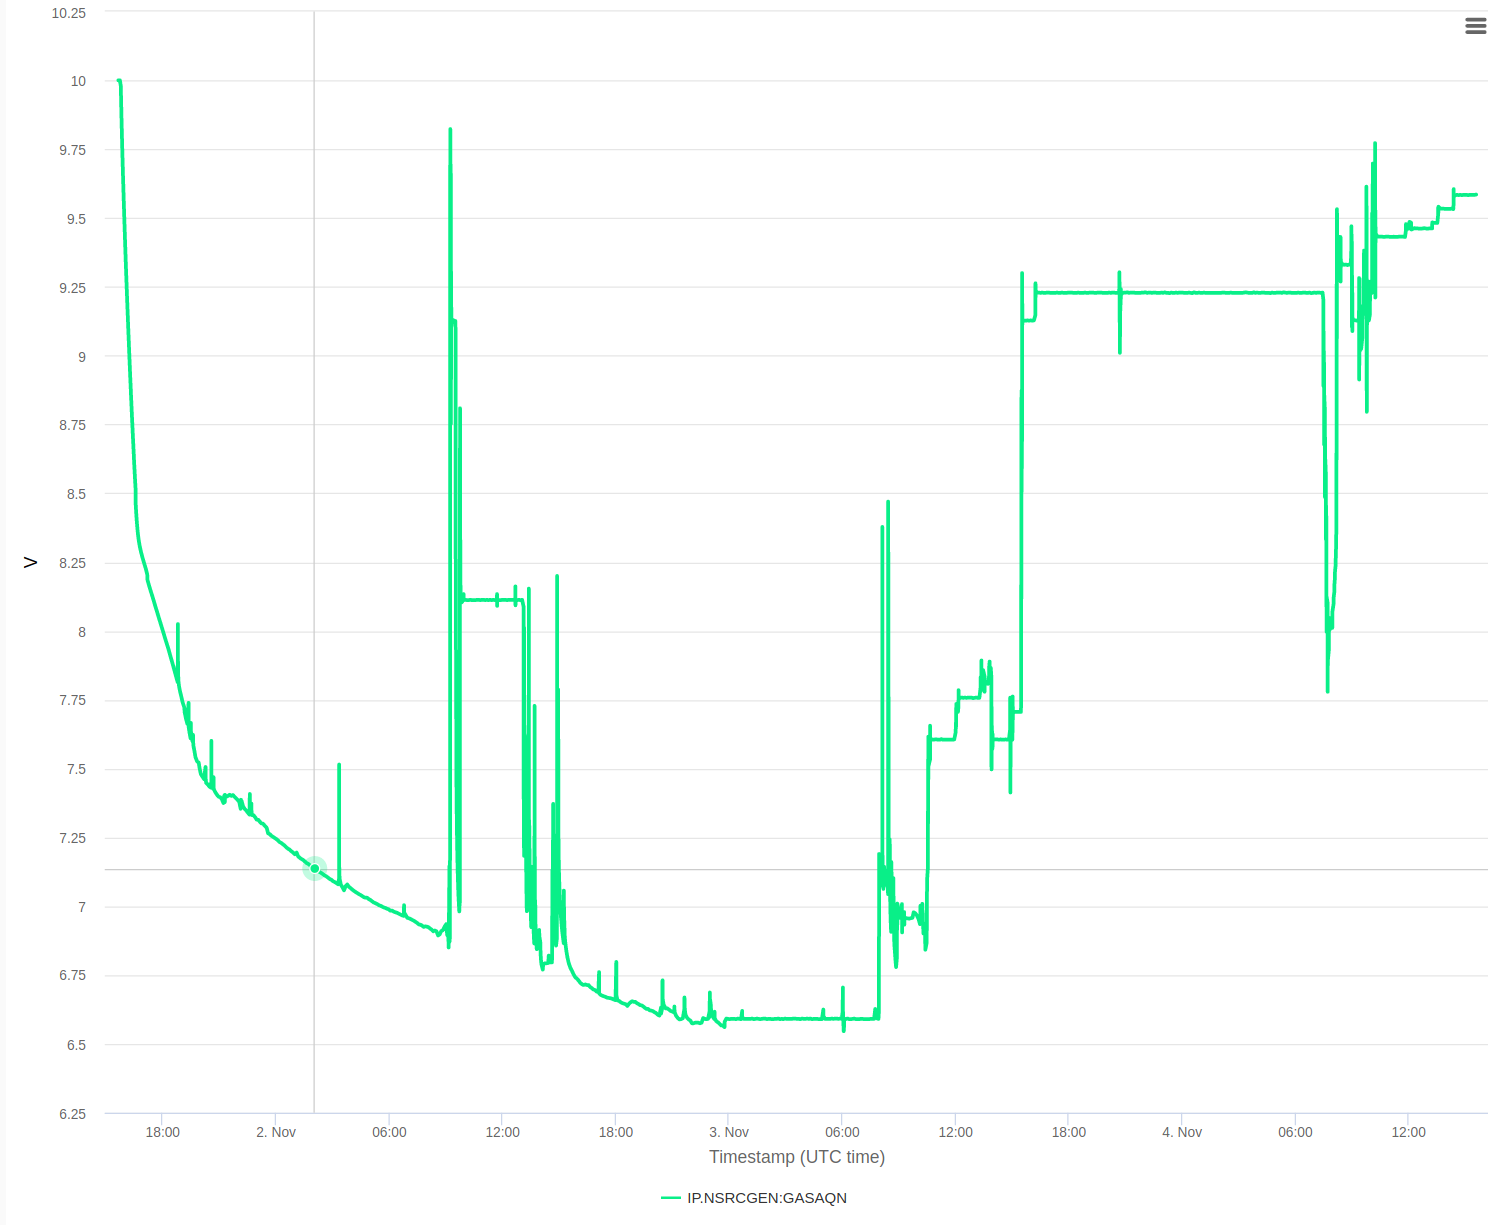
\includegraphics{images/gas_example_02112018.png}
\caption{GASAQN voltage on the second and third November 2018. This was
during an oven refill where the gas pressure changes not as a step
function.}
\end{figure}

Under this assumption we can model a setting as a step function~\cite{Weisstein:StepFunction} 
with added noise, and the problem is to find the step
function. I will call the step function \emph{discretization}, because
we separate our time series into discrete states of a fixed setting.

There are several techniques that could be used to solve such a problem,
and we will discuss some of them
\protect\hyperlink{change-point-detection}{below} in more detail for a
different use case. For this use case I combined a simple rolling window
approach with a decision tree regressor. Some results can be seen below.

\begin{figure}
\centering
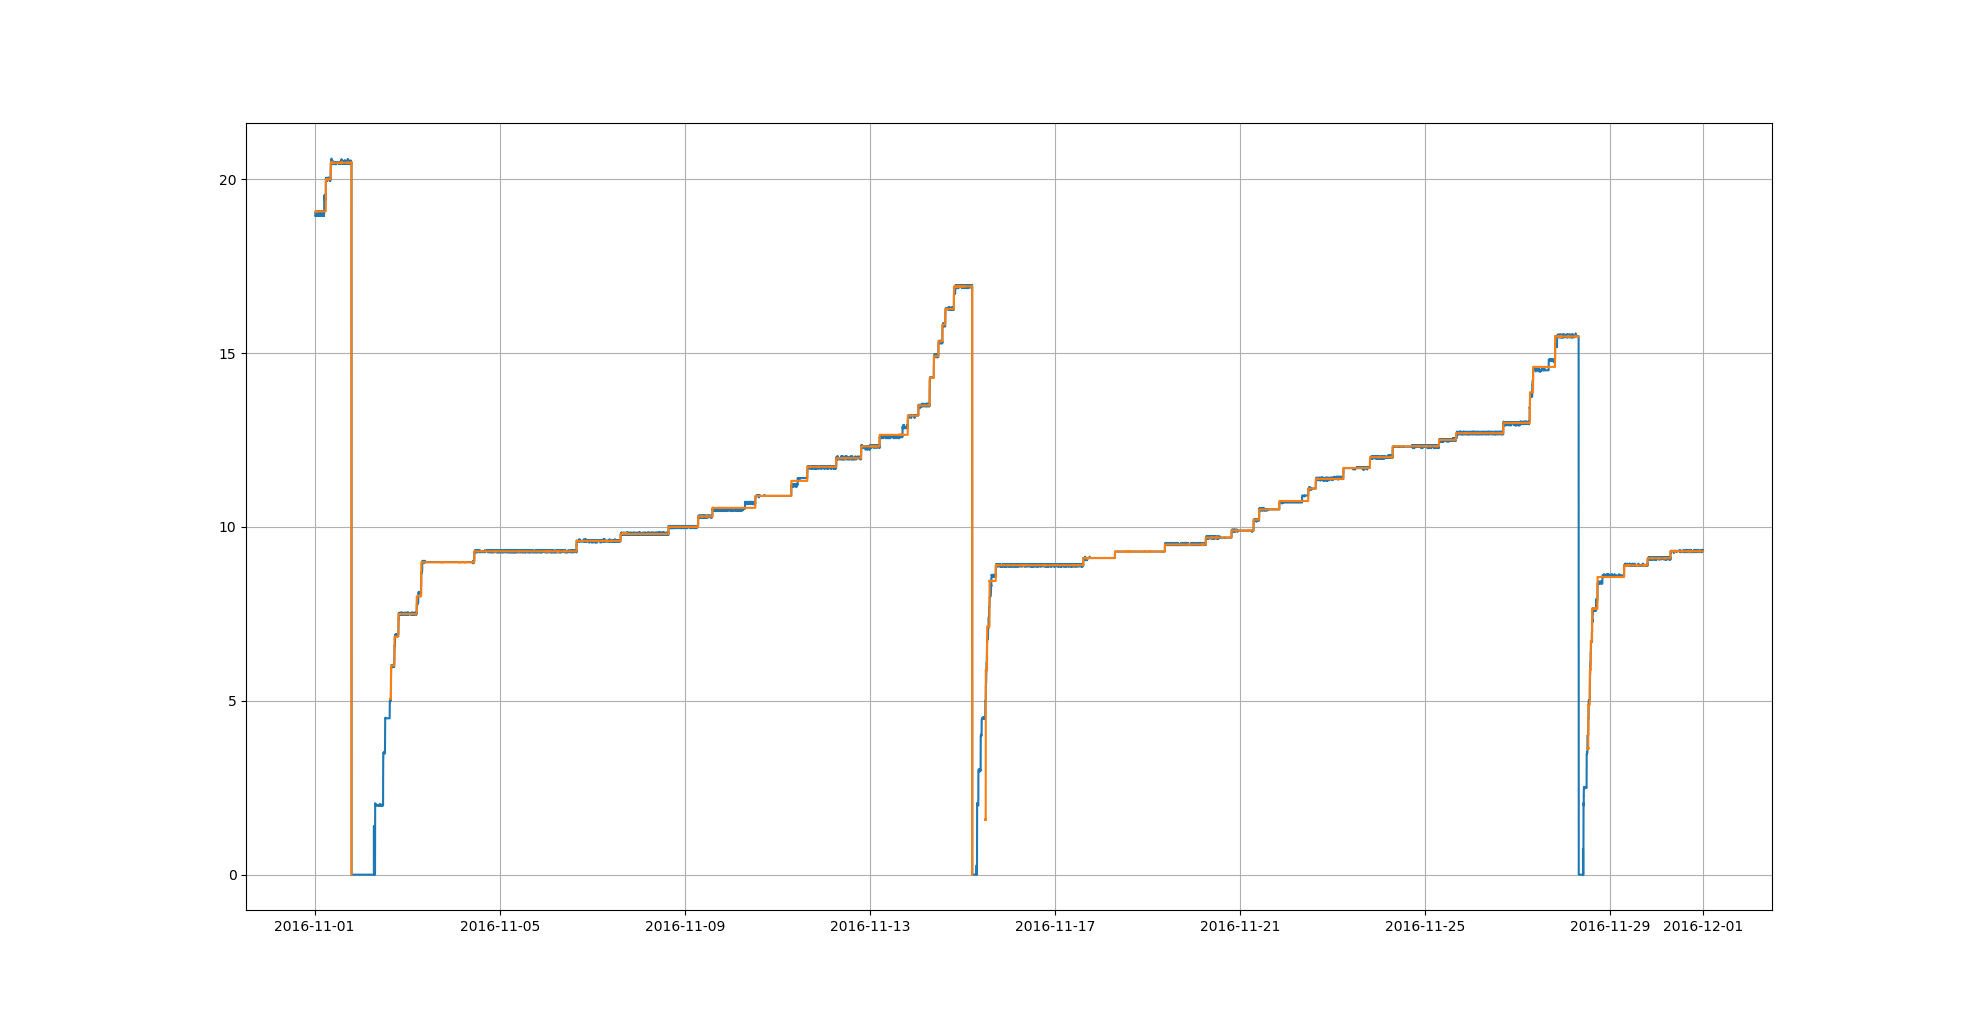
\includegraphics{images/oven_discrete_nov2016.png}
\caption{Discretization of Oven Power for November 2016. In blue the
original data is plotted, the orange line represents the discrete
approximation.}
\end{figure}

\begin{figure}
\centering
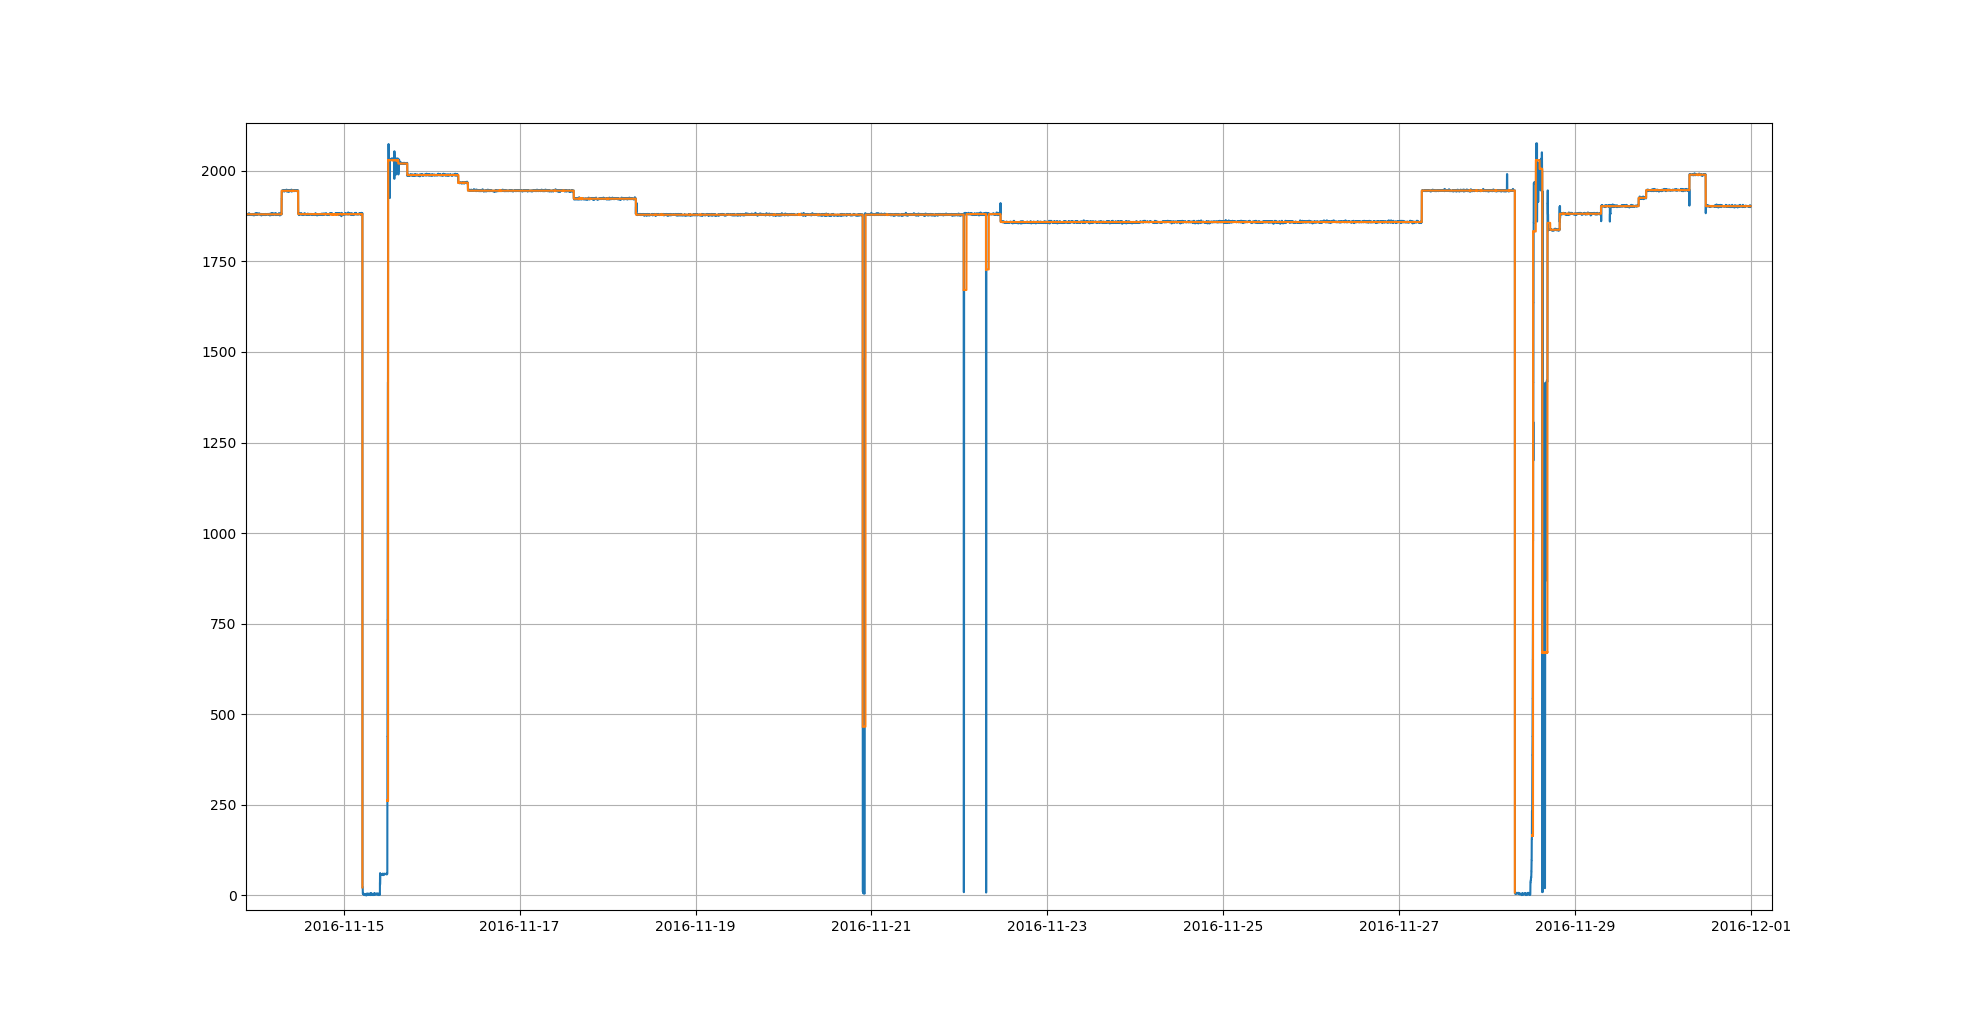
\includegraphics{images/rf_discrete_nov2016.png}
\caption{Discretization of RF Power for November 2016.}
\end{figure}

As one can see, the discrete approximation, our attempt at finding the
true step function, follows the acquisition signal very closely and most
changes are modeled correctly. This can also be seen when comparing the
results with entries in the elogbook (especially for the oven, since
here most changes are noted in the logbook). As can be seen in the
figures, during some periods no discrete approximation is plotted. This
is the case when the source was off (BCT05 current 0A), because the
method does not work well when there are sections with a non-step
function like signal as during an oven restart, so I cut them out.

\hypertarget{explanation}{%
\subsection{Explanation}\label{explanation}}

As described above, the process involves using a Decision Tree
Regressor. A decision tree partitions the input data by sequentially
applying if-then-else rules. It can be thought of as a directed graph,
were every node is one of these rules. End nodes, so called leaves, that
return the class the input is belonging to. Training a decision tree
means finding an optimal set of rules, that explains the training data
as good as possible. {[}TODO: Add reference{]}. Decision trees are a
supervised learning method, meaning that for each training input a
output class is specified, and the algorithm tries to learn this
relationship.

Decision trees can be used for regression. If you want to regress a
function
\(\mathbb R^n \to \mathbb R; \quad (x_1, \dots, x_n) \mapsto y\) you
pass \((x_1, \dots, x_n)\) as input and \(y\) as the desired class. In
the case of an one dimensional function for example, a decision tree
classifier could lern that for \(x>=5\) and \(x<=10\) it should output
\(y=5\). So, by the nature of a decision tree, the regression result is
a step function, that looks like the result as much as possible.

One very common problem with decision trees is over fitting. If they are
allowed to grow too much, they are not regressing any more, but copying.
For example suppose that all your input data points are the natural
numbers. By building a tree with the rules \((x >= 0.5, x <1.5)\),
\((x >= 1.5, x <2.5)\), \((x >= 2.5, x <3.5)\), \ldots{} the resulting
regressor could perfectly replicate the input function, but it would
learn all small oscillations, what is not what we are typically
interested in. However, one thing that can be controlled is how many
leaf nodes the tree can have, i.e.~in the 1D case into how many
intervals the real axis can be split at most.

In our case it would hence be useful to know how many discrete levels,
or number of constant segments, the function we want to model consist
of. Then, we could regress it using a tree with this maximum of leaf
node, because by minimizing the error (i.e.~difference from the original
function) it would find the best stepwise approximation to the input
data without over-fitting.

\hypertarget{finding-the-number-of-constant-segments}{%
\paragraph{Finding the number of constant
segments}\label{finding-the-number-of-constant-segments}}

\hypertarget{change-point-detection}{%
\section{Change Point Detection}\label{change-point-detection}}

\hypertarget{suffix-arrays}{%
\section{Suffix arrays}\label{suffix-arrays}}

\hypertarget{references}{%
\section*{References}\label{references}}
\addcontentsline{toc}{subsection}{References}

\hypertarget{refs}{}
\printbibliography

\end{document}
